\documentclass[a4paper,12pt]{article}
\usepackage[a4paper, margin=2.5cm]{geometry}
\usepackage[pdftex]{graphicx}
\usepackage{tikz}
\usepackage{float}
\usepackage[document]{ragged2e}
\usepackage[utf8]{inputenc}
\usepackage[T1]{fontenc}
\usepackage[spanish,es-tabla]{babel}
\renewcommand{\shorthandsspanish}{}
\usepackage{xurl}
\usepackage{lipsum}
\usepackage{mwe}
\usepackage{multicol}
\usepackage{siunitx}
\usepackage{listings}
\usepackage{circuitikz}
\usepackage{amsmath}

\graphicspath{ {/home/saikkopat/Documents/ESCOM/CE/"Tarea Thevenin"/} }

\title{Tarea 2 tercer parcial: Thévenin}
\author{González Cárdenas Ángel Aquilez}

\begin{document}

\begin{titlepage}
	\begin{tikzpicture}[overlay, remember picture]
		\path (current page.north east) ++(-0.3,-1.5) node[below left] {
\includegraphics[width=0.35\textwidth]{/home/saikkopat/Documents/LOGOS IPN/EscudoESCOM}};
	\end{tikzpicture}
	\begin{tikzpicture}[overlay, remember picture]
		\path (current page.north west) ++(1.5,-1) node[below right] {
\includegraphics[width=0.2\textwidth]{/home/saikkopat/Documents/LOGOS IPN/logo}};
	\end{tikzpicture}
	\begin{center}
		\vspace{-1.5cm}
		{\LARGE Instituto Politécnico Nacional\par}
		\vspace{.5cm}
		{\LARGE Escuela Superior de Cómputo\par}
		\vspace{2.5cm}
		{\large Unidad de aprendizaje:}\\{\Large Circuitos Eléctricos\par}
		\vspace{2cm}
		{\scshape\Huge Tarea:\par}
		{\itshape\Large Teorema de Thévenin\par}
		\vfill
		\vspace{.7cm}
		{\Large Grupo: 3CV2\par}
		\vspace{.7cm}
		{\Large Integrantes:\\González Cárdenas Ángel Aquilez\\Sánchez González Daniel Iván\par}
		\vspace{1cm}
		{\Large Profesor: Vázquez Ortiz Mijail\par}
		\vspace{1cm}
		{\large Fecha de entrega: 6 de junio de 2023\par}
		\vfill
	\end{center}
\end{titlepage} 

\newpage


\section*{Teorema de Thévenin}

Determine el circuito equivalente de Thévenin externo a $R_5$ para el siguiente circuito. Aplique intercambio de fuente y obtenga el circuito equivalente de Norton. Determine el valor de $R_5$ que hace que los circuitos equivalentes transfieran la máxima potencia a dicha resistencia y calcule el valor de esa potencia. Dibuje ambos circuitos equivalentes.\par

\vspace{.5cm}

\begin{figure}[h!]
	\centering
	  \begin{circuitikz}[american, voltage dir=RP] 
	  		\draw	(0,-4) 
	  		to[battery, l=$E$, a=$\SI{10}{\volt}$] (0,4) -- (6,4)
			to[R, a=$R_1$, l=$\SI{10}{\ohm}$] (2,0)
			to[R, a=$R_3$, l=$\SI{20}{\ohm}$] (6,-4) -- (0,-4);
			\draw (6,4)
			to[R, a=$R_2$, l=$\SI{20}{\ohm}$] (10,0)
			to[R, a=$R_4$, l=$\SI{50}{\ohm}$] (6,-4);
			\draw (2,0) -- (4,0) node[anchor=south](A){$A$}
			to[R, a=$R_5$, l=$\SI{30}{\ohm}$,o-o] (8,0) node[anchor=south](B){$B$} -- (10,0);
		\end{circuitikz}
	\caption{Circuito 1}
\end{figure}

\vspace*{-1cm}

\subsection*{Solución}

Primero, para determinar la resistencia equivalente de Thévenin $R_{Th}$, apagamos la fuente de voltaje $E$ y desconectamos la resistencia $R_5$, resultando en el siguiente circuito:


\begin{figure}[h!]
	\centering
	  \begin{circuitikz}[american, voltage dir=RP] 
	  		\draw	(0,-4) -- (0,4) -- (6,4)
			to[R, a=$R_1$, l=$\SI{10}{\ohm}$] (2,0)
			to[R, a=$R_3$, l=$\SI{20}{\ohm}$] (6,-4) -- (0,-4);
			\draw (6,4)
			to[R, a=$R_2$, l=$\SI{20}{\ohm}$] (10,0)
			to[R, a=$R_4$, l=$\SI{50}{\ohm}$] (6,-4);
			\draw (2,0) -- (4,0) node[anchor=south](A){$A$}
			to[ohmmeter,o-o] (8,0) node[anchor=south](B){$B$} -- (10,0);
		\end{circuitikz}
	\caption{Circuito equivalente para determinar $R_Th$}
\end{figure}

Como $( R_2 + R_4 ) || ( R_1 + R_3 )$, tenemos que
\[ (20+50)\SI{}{\ohm} || (10+20)\SI{}{\ohm} = \SI{70}{\ohm} || \SI{30}{\ohm}\]
Así
\[ R_{Th} = \frac{70(30)}{70+30} \SI{}{\ohm} = \SI{21}{\ohm}\]

Luego, para determinar el voltaje del circuito equivalente de Thévenin tenemos el siguiente circuito:

\begin{figure}[h!]
	\centering
	  \begin{circuitikz}[american, voltage dir=RP] 
	  		\draw	(0,-4) 
	  		to[battery, l=$E$, a=$\SI{10}{\volt}$] (0,4) -- (6,4)
			to[R, a=$R_1$, l=$\SI{10}{\ohm}$] (2,0)
			to[R, a=$R_3$, l=$\SI{20}{\ohm}$] (6,-4) -- (0,-4);
			\draw (6,4)
			to[R, a=$R_2$, l=$\SI{20}{\ohm}$] (10,0)
			to[R, a=$R_4$, l=$\SI{50}{\ohm}$] (6,-4);
			\draw (2,0) -- (4,0) node[anchor=south](A){$A$}
			to[voltmeter,o-o] (8,0) node[anchor=south](B){$B$} -- (10,0);
		\end{circuitikz}
	\caption{Circuito equivalente para determinar $E_Th$}
\end{figure}


De la Figura 3 se aprecia que la diferencia de potencial será la diferencia entre los punto A y B, por lo que utilizando la regla del divisor de voltaje se tiene:\par
Para el voltaje en el punto A:
\[ V_A = \frac{\SI{10}{\volt}(\SI{20}{\ohm})}{\SI{30}{\ohm}} = \SI{6.66}{\volt} \]
Para el voltaje en el punto B:
\[ V_B = \frac{\SI{10}{\volt}(\SI{50}{\ohm})}{\SI{70}{\ohm}} = \SI{7.14}{\volt} \]
Luego
\[E_{Th} = V_A - V_B = \SI{-0.48}{\volt} = \SI{-480}{\m\volt} \]
O bien
\[E_{Th} = V_B - V_A = \SI{0.48}{\volt} = \SI{480}{\m\volt} \]

Así, con $R_L = R_5 = \SI{30}{\ohm}$, tenemos el circuito equivalente de Thévenin:


\begin{figure}[h!]
	\centering
	  \begin{circuitikz}[american, voltage dir=RP] 
	  		\draw (0,0)
			to[battery, l=$E_{Th}$, a=$\SI{480}{\m\volt}$] (0,4)
			to[R, l=$R_{Th}$, a=$\SI{21}{\ohm}$] (4,4)
			node[anchor=south](A){$A$} 
			to[R, a=$R_{L}$, l=$\SI{30}{\ohm}$, o-o] (4,0)
			node[anchor=north](B){$B$} -- (0,0);
		\end{circuitikz}
	\caption{Circuito equivalente de Thévenin}
\end{figure}

De donde obtenemos la potencia máxima, resultando en:

\[ P_{Lmax} = \frac{E_{Th}^2}{4(R_{Th})} = \frac{\SI{480}{\m\volt} ^2}{4(\SI{21}{\ohm})} = \SI{2.74}{\m\watt} \]\\

\vspace{1.5cm}

Finalmente, de la Figura 4 obtenemos el circuito equivalente de Norton mediante la conversión de fuente:


\begin{figure}[h!]
	\centering
	  \begin{circuitikz}[american, voltage dir=RP] 
	  		\draw (0,0)
			to[isource, a=$I_N$, l=$\SI{22}{\m\ampere}$] (0,4) -- (3,4)
			to[R, l=$R_{Th}$, a=$\SI{21}{\ohm}$] (3,0) -- (0,0);
			\draw (3,4) -- (6,4) node[anchor=south](A){$A$} 
			to[R, a=$R_{L}$, l=$\SI{30}{\ohm}$, o-o] (6,0)
			node[anchor=north](B){$B$} -- (3,0);
		\end{circuitikz}
	\caption{Circuito equivalente de Norton}
\end{figure}

Con la fuente de corriente obtenida de:
\[ I_N = \dfrac{\SI{480}{\m\volt}}{\SI{21}{\ohm}} \approx \SI{0.02285}{\ampere} = \SI{22}{\m\ampere} \]

\newpage


\section*{Simulaciones}

Las siguientes simulaciones se realizaron utilizando el simulador multiplataforma EveryCircuit\texttrademark.\par



\vspace{.5cm}

\begin{figure}[!h]
\centering
	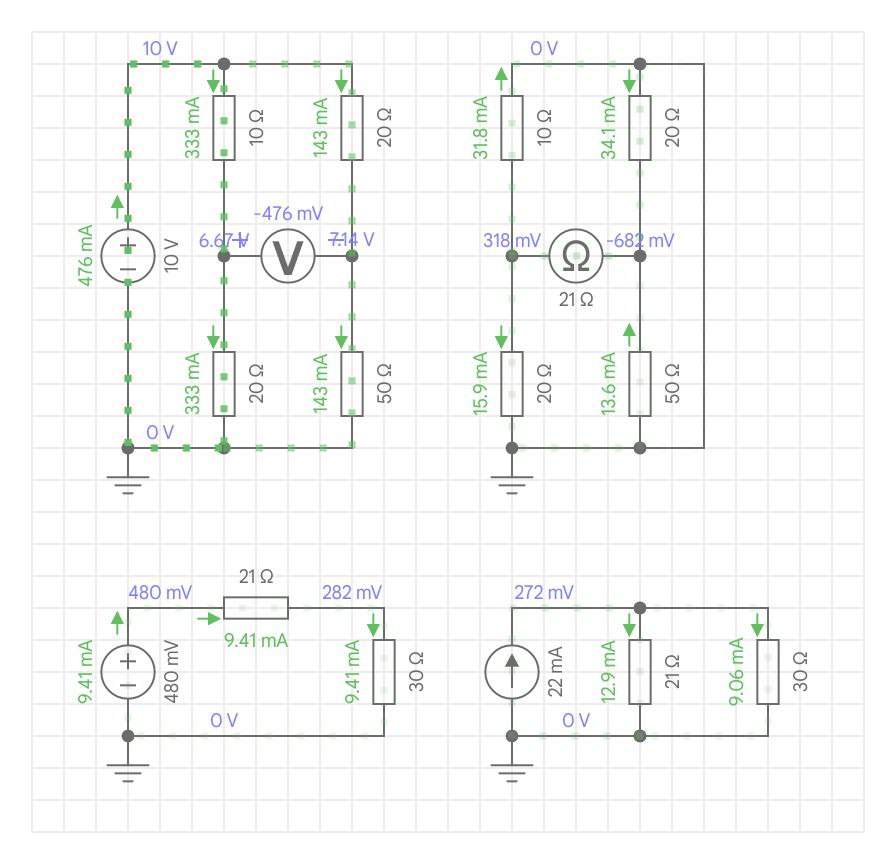
\includegraphics[width=.8\textwidth]{fig1}
	\label{fig1}
	 \caption{Simulaciones de los circuitos}
\end{figure}


\end{document}